
One of the most common and intuitive approaches for implementation of software controller for hardware system is state-machine approach. It is fairly simple concept, with only a couple of important considerations.

System controlled by state machine has certain number of possible, unique and well defined states that it can be in at every moment of execution. State defines the behaviour of the system in every discrete moment of time, including three important aspects: sensor data acquisition, output behaviour computation and state transition check. In other words, every state has it is own logic for doing all of these three mentioned steps, which gives a lot of variability for possible control scenarios. It is worth mentioning that some states might skip certain steps or perform some steps more than once without state transition check, for example.

\paragraph{System states}

At any moment of time robot can be in one of the following state seen in figure \ref{fig:algorithm-diagram}.

\begin{figure}[ht!]
	\centering
	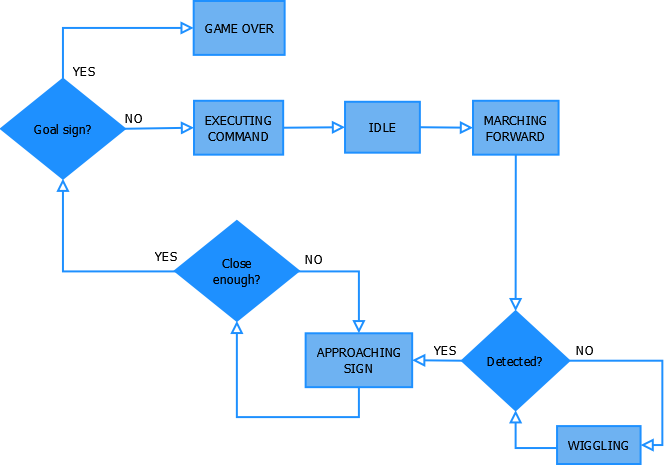
\includegraphics[width=0.7\textwidth]{newDiagram.png}
	\caption{State transition algorithm}
	\label{fig:algorithm-diagram}
\end{figure}

\textit{IDLE} state sets both angular and linear speed to zero and waits for any of the segmented object currently inside view to go away, after which it goes to WIGGLING state.

\textit{WIGGLING} state rotates the robot around its vertical axis with constant angular and zero linear speed until a sign is detected. After detecting a sign it switches to APPROACHING\_SIGN state.

\textit{APPROACHING\_SIGN} state moves the robot close to the sign it has seen in the previous state. It does this by setting the linear speed to constant value and adjusting angular speed all the time based on the horizontal position of the target sign in the view. Robot will move in the direction needed to align the sign to the center of the screen, and it will do that proportionally to the distance of the target to the center.

\textit{EXECUTING\_COMMAND} state has different behavior depending on the type of the sign that was seen in the state before. If it was goal sign, it will switch to the GAME\_OVER state and the game will end. If it was stop sign, robot will just wait for certain predefined time-out (5 seconds) and switch to state MARCHING\_FORWARD. If it was the arrow sign, robot will turn desired angle and switch switch to state MARCHING\_FORWARD.

\textit{MARCHING\_FORWARD} state sets the linear speed to constant and angular to zero. In this state robot constantly monitors camera image stream and can potentially switch to APPROACHING\_SIGN state once a sign is detected in perceptive area of the image.

\textit{GAME\_OVER} state is entered after goal sign is approached. After displacing notification about game completion (through audio and visual feedback), robot remains idle until hardware button is pressed for the start of the new game.

%\begin{figure}[th!]
%	\centering
%	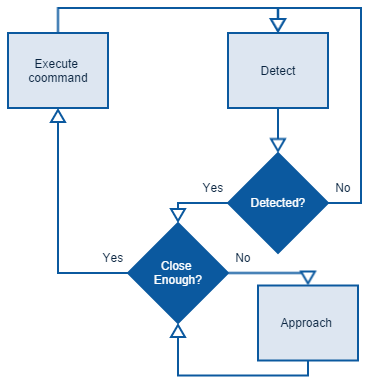
\includegraphics[scale=1]{algorithm-diagram.png}
%	\caption{State transition algorithm}
%	\label{fig:algorithm-diagram}
%\end{figure}

%\paragraph{Sensor data acquisition}

First step in state machine control loop is sensor acquisition step. If possible, data is acquired from all input sensors in order to determine current state of the environment. This includes acquisition of camera image using OpenCV, reading heading angle from motor driver and reading distances from ultrasonic sensor driver.

Last values of all the readings are always stored in local members of the class, so they can be referenced between successive acquisitions.

%\paragraph{Output behavior computation}

Based on the sensed input data values for all output units are being calculated. This includes linear and angular wheel velocities, message for LCD display, sound to be played on speakers, etc.

%\paragraph{State transition condition}

Every state has to have clearly defined condition which will make the system switch to any of the other states. System remains in the current state until one of the state transition conditions has been met.



